%!TEX encoding = UTF8
%!TEX root =notes.tex

\chapter{Droite réelle et géométrie plane}

\section{Droite réelle}
	

On considère la droite graduée suivante.

\begin{center}
	
	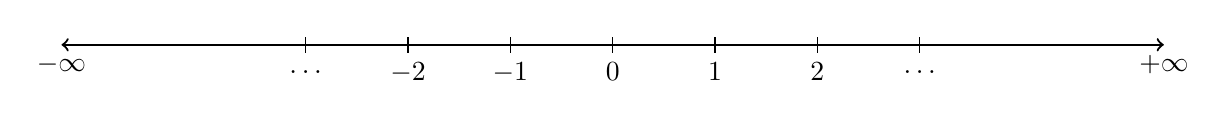
\begin{tikzpicture}
		
		% real line
		\draw[<->, thick] (-7,0) node[below] {$-\infty$} -- (7,0) node[below] {$+\infty$};
		
		\foreach \x in {-2,...,2}
			\draw[-] (1.3*\x,-.1) node[below] {$\x$} -- (1.3*\x,.1) node{};
		
		\foreach \x in {-3, 3}
			\draw[-] (1.3*\x,-.1) node[below=3pt] {$\dots$} -- (1.3*\x,.1) node{};
		
	
	\end{tikzpicture}
\end{center}

On peut construire à la règle et au compas le nombre $\sqrt{2}$ sur la droite grâce au théorème de Pythagore.

\exe{}{
	Construire, en utilisant uniquement la règle et le compas, tous les nombres rationnels, c'est-à-dire toutes les fractions $\dfrac{p}q$ où $p, q \in \Z$ et $q \neq 0$.
	
	\emph{Indication : les couples $(1, p/q)$ et $(q, p)$ sont proportionnels.}
}{}

L'ensemble des points de la droite est donc strictement plus grand que celui des rationnels, car $\sqrt{2}$ n'est pas rationnel d'après le théorème \ref{thm:1}.

\begin{center}
	
	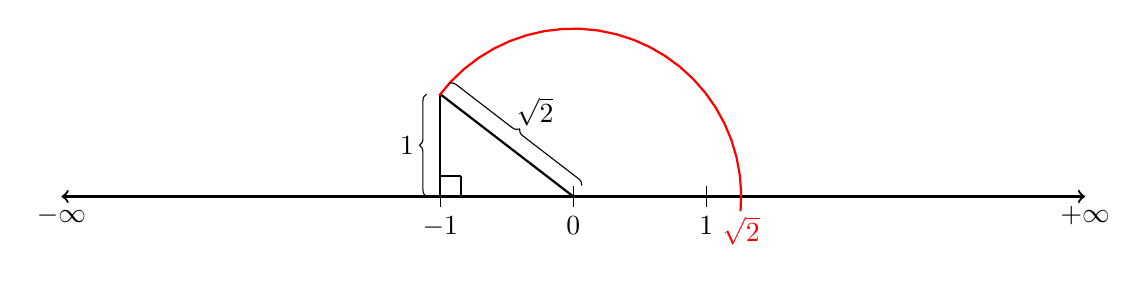
\begin{tikzpicture}[scale=1.3]
		
		% real line
		\draw[<->, thick] (-5,0) node[below] {$-\infty$} -- (5,0) node[below] {$+\infty$};
		\foreach \x in {-1, 0, 1}
			\draw[-] (1.3*\x,-.1) node[below] {$\x$} -- (1.3*\x,.1);
		
		% right angled triangle
		\draw[-, thick] (-1.3,0) -- (-1.3,1);
		\draw[-, thick] (0,0)-- (-1.3,1);
		
		\draw[-, thick] (-1.1,0)-- (-1.1,.2);
		\draw[-, thick] (-1.1,.2)-- (-1.3,.2);
		
  			
		% circle arc
		 \draw [red,thick,domain=-5:143] plot ({sqrt(2.69)*cos(\x)}, {sqrt(2.69)*sin(\x)});
		 
		 % sqrt{2} mark
		\draw[-, red] (1.640,-.1) node[below, red] {$\sqrt{2}$} -- (1.640,.1);
		
		% lengths
		\draw[decoration={brace,raise=5pt, mirror},decorate]
  			(0,0) -- node[above=12pt, right] {$\sqrt{2}$} (-1.3,1);
		\draw[decoration={brace,raise=5pt},decorate]
  			(-1.3,0) -- node[left=6pt] {$1$} (-1.3,1);
  			
				
	\end{tikzpicture}
\end{center}

Tous les points de la droite ne peuvent en fait pas être construit à la règle et au compas. Ceci est étroitement lié au théorème de Gauss-Wantzel sur les	polygônes réguliers constructibles.
En particulier, l'heptagone régulier n'est pas constructible à la règle et au compas.
	
Ce théorème est en dehors du champ d'application du cours.

\dfn{Nombres réels $\R$}{
	À chaque point de la droite on associe un nombre, appelé \emph{réel}.
	L'ensemble des nombres réels est noté $\R$.
}{}

\nt{
	On a la suite d'inclusions suivantes :
		\[ \N \subset \Z \subset \D \subset \Q \subset \Q. \]
}

\subsection{Intervalles}

\dfn{Intervalle borné}{
	Un intervalle borné est un segment de la droite réelle $\R$. C'est donc un ensemble de nombres.
	Il est donné par une \emph{borne inférieure} $a \in \R$ et une \emph{borne supérieure} $b\in\R$ et peut contenir ou non ses bornes.
	
	\begin{enumerate}
		\item Si $a$ et $b$ sont contenues dans l'intervalle, on le note $[a ; b]$.
		\item Si $a$  est contenue dans l'intervalle mais $b$ ne l'est pas, on le note $[a ; b [$.
		\item Si $a$ n'est pas contenue dans l'intervalle mais $b$ l'est, on le note $] a ; b]$.
		\item Si ni $a$ ni $b$ ne sont contenues dans l'intervalle, on le note $] a ; b [$.
	\end{enumerate}
}{}
\ex{}{
	Les intervalles suivants sont bornés.
	\begin{multicols}{2}
	\begin{enumerate}[label=$\bullet$]
		\item $[-1 ; 1]$
		\item $[-3 ; 1[$
		\item $\left]-10{,}341 ; \pi\right]$
		\item $\left]\sqrt{2} ; 130\right[$
	\end{enumerate}
	\end{multicols}

}{}

\dfn{Intervalle non borné}{
	Un intervalle n'est pas forcément borné : une ou les deux bornes peuvent être infinies ($\pinfty$ ou $\minfty$). 
	Dans ce cas, l'intervalle n'inclut jamais l'infini car ce n'est pas un nombre.
}{}

\ex{}{
	Les intervalles suivants ne sont pas bornés.
	\begin{multicols}{2}
	\begin{enumerate}[label=$\bullet$]
		\item $]\minfty; 2]$
		\item $]\minfty ; 3[$
		\item $]0; \pinfty[$
		\item $\R = ]\minfty; \pinfty[$
	\end{enumerate}
	\end{multicols}
}{ex:3.5}

\subsection{Intersection et union}

\dfn{Intersection, union}{	
	Pour deux ensembles $E, F$ on définit les ensembles suivants.
		\begin{enumerate}
			\item $E \cap F$ : l'intersection des deux ensembles.
			
			Un élément appartient à $E \cap F$ dès qu'il appartient à $E$ \textbf{et} à $F$.
			\item $E \cup F$ : l'union des deux ensembles.
			
			Un élément appartient à $E \cup F$ dès qu'il appartient à $E$ \textbf{ou} à $F$.
		\end{enumerate}
}{}


\exe{}{
	Exprimer les intersections et unions suivantes sous forme d'intervalle.
	\begin{multicols}{2}
	\begin{enumerate}
		\item $[-1 ; 1] \cap [-3 ; 1]$
		\item $] {-}\infty ; 2] \cap [-3 ; -2]$
		\item $]{-}\infty ; 4 [ \cup [2 ; +\infty[$
		\item $]-2 ; 4 [  \cup [4 ; 8[$
	\end{enumerate}
	\end{multicols}
}{ex:inter-union}

\nt{
	Lorsqu'on prend l'intersection de deux intervalles, seules les bornes les plus restrictives subsistent.
	En effet, un nombre appartient à un intervalle si et seulement s'il est à la fois supérieur à la borne inférieure, et inférieur à la borne supérieure (inégalités larges ou strictes à préciser).
	
	Dès lors, pour qu'un élément appartienne à l'intersection de deux intervalles, il doit
		\begin{enumerate}
			\item être supérieur aux deux bornes inférieures, et
			\item être inférieur aux deux bornes supérieures.
		\end{enumerate}
	La plus restrictive des bornes inférieures est donc la plus grande, et la plus restrictive borne supérieure est la plus petite.
	On en déduit une règle générale
		\[ [a ; b] \cap [c ; d] = [ \max\{a, c\} ; \min\{b, d\}]. \]
}

\nt{
	Pour l'union de deux intervalles, les bornes les moins restrictives restent, et on a
		\[ [a ; b] \cup [c ; d] = [ \min\{a, c\} ; \max\{b, d\}]. \]
}

\exe{}{
	Refaire l'exercice \ref{ex:inter-union} à l'aide des règles des remarques ci-dessus.
	Comparer les résultats.
}{}

\subsection{Inégalités}

Un intervalle n'a de sens que si la borne inférieure est plus petite que la borne supérieure.
De plus, un élément appartient à l'ensemble dès qu'il est plus petit que la borne supérieure, et plus grand que la borne inférieure.

Il faut donc pouvoir noter simplement les relations \og plus petit que \fg et \og plus grand que \fg.

\dfn{Inégalités}{
	On définit les signes suivants correspondant à des inégalités \emph{strictes} et \emph{larges}.
		\begin{enumerate}
			\item $<$ : strictement inférieur à
			\item $\leq$ : inférieur ou égal à
			\item $>$ : strictement supérieur à
			\item $\geq$ : supérieur ou égal à
		\end{enumerate}
}{}

%TEMPORARY
\newpage

\ex{}{
	\begin{multicols}{3}
	\begin{enumerate}
		\item $1 \leq 2$
		\item $-3 \leq -2$
		\item $0 \leq 0$
		\item $1{,}02 < 1{,}1$
		\item $7{,}391 > 7{,}30001$
		\item $-4{,}001 > -4{,}0001$
	\end{enumerate}
	\end{multicols}
}{}

\nt{
	Appartenir à un intervalle est donc équivalent à respecter certaines inégalités.
	En particulier : être inférieur à la borne supérieure, et être supérieur à la borne inférieure.
	
	On a donc l'équivalence suivante.
		\[ x \in [a ; b] \qquad \iff \qquad x \in \R, x \geq a, \textbf{ et } x \leq b. \]
		
	On peut noter deux inégalités sur la même lignes dès qu'elles vont dans le même sens.
	Par exemple, les deux inégalités ci-dessus peuvent être condensées en une :
		\[ x \in \R, \text{ et } a \leq x \leq b, \]
	ou encore
		\[ x \in \R, \text{ et } b \geq x \geq a. \]
}

\ex{}{
	\begin{enumerate}
		\item Prendre $x \in [-3 ; 4]$ est équivalent à prendre $x \in \R$ vérifiant $-3 \leq x \leq 4$.
		\item Prendre $x \in [-4 ; 3[$ est équivalent à prendre $x \in \R$ vérifiant $-4 \leq x < 3$.
		\item Prendre $x \in ]\minfty ; 0[$ est équivalent à prendre $x \in \R$ vérifiant $x < 0$.
		
		On dit alors que $x$ est strictement négatif.
		\item Prendre $x \in [0; \pinfty [$ est équivalent à prendre $x \in \R$ vérifiant $x \geq 0$.
		
		On dit alors que $x$ est positif ou nul.
		\item Prendre $x \in ]\minfty; \pinfty[$ est équivalent à prendre $x \in \R$.	
		
		Ceci est en fait tautologique car $]\minfty; \pinfty[ = \R$, comme vu dans l'exemple \ref{ex:3.5}.
	\end{enumerate}
}{}

\thm{}{
	Soient $x, y, a \in \R$ vérifiant
		\[ x \leq y. \]
	Alors l'inégalité ci-dessus est équivalente aux inégalités suivantes.
		\begin{enumerate}
			\item $x + a \leq y + a$, sans condition sur $a$.
			\item $a x \leq a y$ si $a > 0$ est strictement positif.
			\item $ax \geq a y$ si $a < 0$ est strictement négatif.
		\end{enumerate}
}{thm:ineg}
\pf{Justifications du théorème \ref{thm:ineg}}{
	Le point $1.$ se justifie sans peine avec un dessin : ajouter $a$ revient à décaler les points $x$ et $y$ de la droite réelle vers la droite (si $a >0$) ou la gauche (si $a<0$) d'une même distance. 
	Leur relation d'ordre reste donc inchangée.
	
	Étant donné $1.$, on a que $x \leq y$ est équivalent à $y-x \geq 0$.
	Ainsi $y-x$ est un nombre réel positif.
	Or, multiplier deux positifs entre eux donne un nombre positif, et multiplier un nombre négatif avec un positif donne un nombre négatif.
	
	Par conséquent, si $a > 0$, on a bien
		\[ a \cdot (y-x) \geq 0 \iff ay \geq ax \iff ax \leq ay, \]
	et si $a < 0$, on a
		\[ a \cdot (y-x) \leq 0 \iff ay \leq ax \iff ax \geq ay, \]
	ce qui conclut.

}

\nt{
	Le théorème \ref{thm:ineg} reste vrai si on remplace l'inégalité large $\leq$ par une inégalité stricte $<$.
	
	En outre, échanger le rôle de $x$ et de $y$ revient à inverse le sens de l'inégalité.
}

\str{
	On décrit ci-après la stratégie de résolutions d'inéquations du type
		\[ a x + b \leq c x + d, \]
	où $a,b,c,d \in \R$ sont des réels quelconques et $x\in\R$ est l'inconnue à placer dans un intervalle.
	
	Comme pour les équations, on procède en deux étapes
		\begin{enumerate}
			\item Isoler les multiples de $x$ d'un côté et les constantes de l'autre.
			\item Diviser pour trouver l'intervalle de $x$.
		\end{enumerate}
	Pour cela, on peut par exemple soustraire $cx$ et $b$ des deux côtés à l'aide du Théorème \ref{thm:ineg}.
		\[ (a-c) x \leq d - b.\]
	Si $a-c \neq 0$, on divise par $a-c$ en faisant attention au signe de celui-ci :
		\[ \begin{cases*} 
						x \leq \dfrac{d-b}{a-c} & si $a-c > 0$, \\
					 	x \geq \dfrac{d-b}{a-c} & si $a-c < 0$.
			\end{cases*} \]
}

\ex{}{
	Essayons de déterminer quels réels $x\in\R$ vérifient l'inégalité suivante.
		\[ 3 x + 1 \geq  8 \]
	Cette inégalité est équivalente à
		\begin{align*}
			 3x \geq 7,  && \text{puis à} && x\geq \dfrac73,
		\end{align*}			
	car $\frac13 > 0$ est strictement positif et d'après le théorème \ref{thm:ineg}.
	
	On a donc trouvé que
		\[ \{ x \in \R \text{ tq. } 3x + 1 \geq 8 \} = \left[\dfrac73 ; \pinfty\right[. \]
}{}

\ex{}{
	On détermine les réels $x \in \R$ vérifiant la double inégalité suivante.
		\[ 14 > - 7x + 10 \geq -1.\]
	On vérifie d'abord qu'on ait $14 > -1$ pour s'assurer que de tels réels $x$ existent bien. 
	On peut par exemple résoudre l'équation $-7x+10 = 2$ pour avoir un exemple d'un tel $x$ (car $14 > 2 \geq -1$).
	
	L'inégalité est équivalente à
		\[ 4 > -7x \geq -11. \]
	On divise ensuite par $-7$, ce qui échange le sens des inégalités car $\dfrac{1}{-7}$ est strictement négatif.
	D'où
		\[ \dfrac{4}{-7} < x \leq  \dfrac{-11}{-7}. \]
	Finalement, on a obtenu que
		\[ \{ x \in \R \text{ tq. } 14 > - 7x + 10 \geq -1 \} = \left]{-}\dfrac47 ; \dfrac{11}7\right]. \]
}{}

\exe{}{
	Trouver quels réels $x\in\R$ vérifient les deux inégalités suivantes
		\begin{align*} -\dfrac32x - 2 \geq -4 && \textbf{et} && -\dfrac32x -2 \leq 13 & \end{align*}
	en prenant l'intersection des intervalles obtenus pour chaque inégalité.
	
	Faire de même en manipulant directement la double inégalité
		\[ -4 \leq -\dfrac32x -2 \leq 13, \]
	et vérifier qu'on trouve le même intervalle final.
}{}



\subsection{Valeur absolue}

La valeur absolue correspond à la notion de \emph{distance} parmis les réels.
Celle-ci intervient notamment lorsqu'on souhaite calculer la longueur d'un intervalle borné afin de mesure sa précision.
Par exemple, l'intervalle $[1 ; 3]$, dans lequel $2$ appartient, est moins précis que l'intervalle $[1{,}99 ; 2{,}01]$ car sa longueur est plus grande.

Les intervalles de confiance seront étudiés plus tard dans le chapitre dédié aux statistiques.

\exe{}{
	Quelle est la distance dans les réels 
		\begin{multicols}{2}
		\begin{enumerate}
			\item $3$ et $2$ ?
			\item $2$ et $4$ ?
			\item $-1$ et $1$ ?
			\item $-4{,}2$ et $-4{,}12$ ?
		\end{enumerate}
		\end{multicols}
}{}

\dfn{Valeur absolue}{
	La valeur absolue d'un $x \in \R$ général est égale à $x$ si celui-ci est positif, et à son opposé $-x$ sinon.
	La valeur absolue est donc toujours positive et peut être définie comme suit.
	
		\[ |x| = \begin{cases} x \text{ si $x \geq 0$}, \\ -x \text{ sinon.} \end{cases}. \]

	Soient $a, b \in \R$ deux réels quelconques.
	La distance de $a$ à $b$ est égale à
		\[ \text{Distance entre $a$ et $b$} = \begin{cases} a-b \text{ si $a \geq b$} , \\ b-a \text{ sinon.} \end{cases}. \]
	La condition $a \geq b$ peut être réécrite comme $a-b \geq 0$.
	
	En remarquant que $b-a = -(a-b)$, on voit que la distance entre $a$ et $b$ est exactement donnée par la valeur absolue de $a-b$.
		\[ \text{Distance entre $a$ et $b$} = | a- b|. \]
}{}

\nt{
	On retrouve d'ailleurs $|x| = |x - 0|$, la distance de $x$ à $0$.
}

\str{
	Pour résoudre une équation du type
		\[ |E| = a, \]
	où $E$ est une certaine expression, et $a\in\R$ est un nombre réel positif ou nul, on remarque que l'égalité est équivalente à
		\begin{align*}
			E = a, && \text{ ou } && E = -a.
		\end{align*}
}

\ex{}{
	On cherche un réel $x\in\R$ vérifiant l'égalité
		\[ |3x-8| = 5. \]
	En comprenant $3x-8$ comme l'expression $E$ et $5$ comme le réel $a$ de la stratégie ci-dessus, on se retrouve à résoudre les deux équations linéaires suivantes.
		\begin{align*}
			3x-8 = 5, && \text{ ou } && 3x-8 = -5.
		\end{align*}
	On les résoud calmement pour trouver
		\begin{align*}
			x = \dfrac{13}3, && \text{ ou } && x = 1.
		\end{align*}
	On pourra alors vérifier les valeurs obtenues en substituant dans l'équation d'origine.
	On a bien
	
		\begin{align*}
			|3 \times \dfrac{13}3 - 8| = |5| =5, && \text{ et } && |3 \times 1 - 8| = |-5| =5,
		\end{align*}
	ce qui nous rassure.
}{}

\str{
	Pour résoudre une inéquation du type
		\[ |E| \leq a, \]
	où $E$ est une certaine expression, et $a\in\R$ est un nombre réel positif ou nul, on remarque que l'inégalité est équivalente à
		\begin{align*}
			- a \leq E \leq a.
		\end{align*}
	Le résultat donnera donc un intervalle.
		
	On fera attention au caractère stricte ou non des inégalités en question.
}

\ex{}{
	On cherche quels réels $x\in\R$ vérifient l'inégalité
		\[ |2x-3| < 1. \]
	En comprenant $2x-3$ comme l'expression $E$ et $1$ comme le réel $a$ de la stratégie ci-dessus, on se retrouve à résoudre les inégalités strictes suivantes. 
		\[
			-1 < 2x-3 < 1.
		\]
	On les résoud pour trouver
		\[
			\{ x \in \R \text{ tq. } |2x-3| < 1 \} = \{ x \in \R \text{ tq. } 1 < x < 2 \} = ]1; 2[.
		\]
	On pourra alors s'assurer que n'importe quel $x\in\R$ réel de l'intervalle $]1;2[$ vérifie bien que $|2x-3|<1$, par exemple en testant quelques valeurs (dont les bornes).
}{}

\exe{}{
		Quels réels $x\in\R$ vérifient les conditions suivantes ? Donner des ensembles finis ou des intervalles.
		\begin{multicols}{2}
		\begin{enumerate}
			\item $|x| = 1$
			\item $|2x -4| = 5$
			\item $| x | \leq 3{,}14$
			\item $| 7 + 3x | \leq 10$
		\end{enumerate}
		\end{multicols}
}{}

\str{
	Pour résoudre une inéquation du type
		\[ |E| \geq a, \]
	où $E$ est une certaine expression, et $a\in\R$ est un nombre réel positif ou nul, on remarque que l'inégalité est équivalente à
		\begin{align*}
			E \leq -a, && \text{ ou } && E \geq a.
		\end{align*}
	Le résultat donnera donc une union de deux intervalles.
		
	On fera également attention au caractère stricte ou non des inégalités en question.
}

\ex{}{
	On cherche quels réels $x\in\R$ vérifient l'inégalité
		\[ \left|5 - \dfrac12x \right| \geq 3. \]
	En comprenant $5 - \dfrac12x$ comme l'expression $E$ et $3$ comme le réel $a$ de la stratégie ci-dessus, on se retrouve à résoudre les inégalités strictes suivantes. 
		\begin{align*}
			5 - \dfrac12x \leq -3, && \text{ ou } && 5 - \dfrac12x \geq 3.
		\end{align*}
	On les résoud pour trouver
		\[
			\{ x \in \R \text{ tq. }  \left|5 - \dfrac12x \right| \geq 3 \} = \{ x \in \R \text{ tq. } x \geq 16 \text{ ou } x \leq -4\} = ]\minfty ; -4] \cup [16; \pinfty[.
		\]
}{}

\nt{
	Il sera pratique à partir de maintenant de noter la multiplication de deux nombres par le point médian $\cdot$ à la place de la croix $\times$ pour la distinguer plus facilement du réel $x$.
	
	La notation $\times$ prendra d'autres sens en mathématiques plus tard : produit cartésien, produit vectoriel (notation anglosaxone), dimensions de matrices, etc…
}

\thm{Propriétés de la valeur absolue}{
	Soient $x,y\in\R$ deux nombres réels quelconques.
	Alors
		\begin{enumerate}
			\item $|x| = \left|-x\right|$
			\item $|x \cdot y| = |x| \cdot |y|$
			\item $\sqrt{x^2} = |x|$
		\end{enumerate}
}{}